\newcommand{\decktitle}{Grundlagen der Informatik}
%%%%%%%%%%%%%%%%%%%%%%%%%%%%%%%%%%%%%%%%%%%%%%%%%
%
% DOCUMENT
%
%%%%%%%%%%%%%%%%%%%%%%%%%%%%%%%%%%%%%%%%%%%%%%%%%

\begin{frame}
    \subtitle{\decktitle}
    \titlepage
\end{frame}


\begin{frame}
    \frametitle{\textbf{Outline:}}
    \tableofcontents
\end{frame}


		
  
\section{Grundlagen der Informatik}  
    \subsection{Definition}
    
    \begin{frame}{Was ist Informatik?}
        \begin{definition}
         \begin{quote}
            Wissenschaft von der systematischen Darstellung, Speicherung, Verarbeitung und Übertragung von Informationen, besonders der automatischen Verarbeitung mithilfe von Digitalrechnern \cite{claus2006duden}
            \end{quote}  
        \end{definition}
        
    \end{frame}
          
    \begin{frame}{Was ist Informatik?}
        Informatik setzt sich als Kofferwort aus den zwei Bereichen \alert{Information} und \alert{Automatik} zusammen. 
        \\[2\baselineskip]
        
        Es geht also um \textit{automatisierte Informations- / Datenverarbeitung}. Beide Teilbereiche sind elementar wichtig und werden im Rahmen dieser Veranstaltung direkt und indirekt näher beleuchtet.
    \end{frame}
    
    \subsection{Teilbereiche der Informatik am Beispiel Google}
    
    \begin{frame}{Was ist Informatik?}
    \framesubtitle{Beispiel Google: Programmierung}
     \begin{columns}
        \begin{column}{0.5\textwidth}
            \begin{figure}
                \centering
                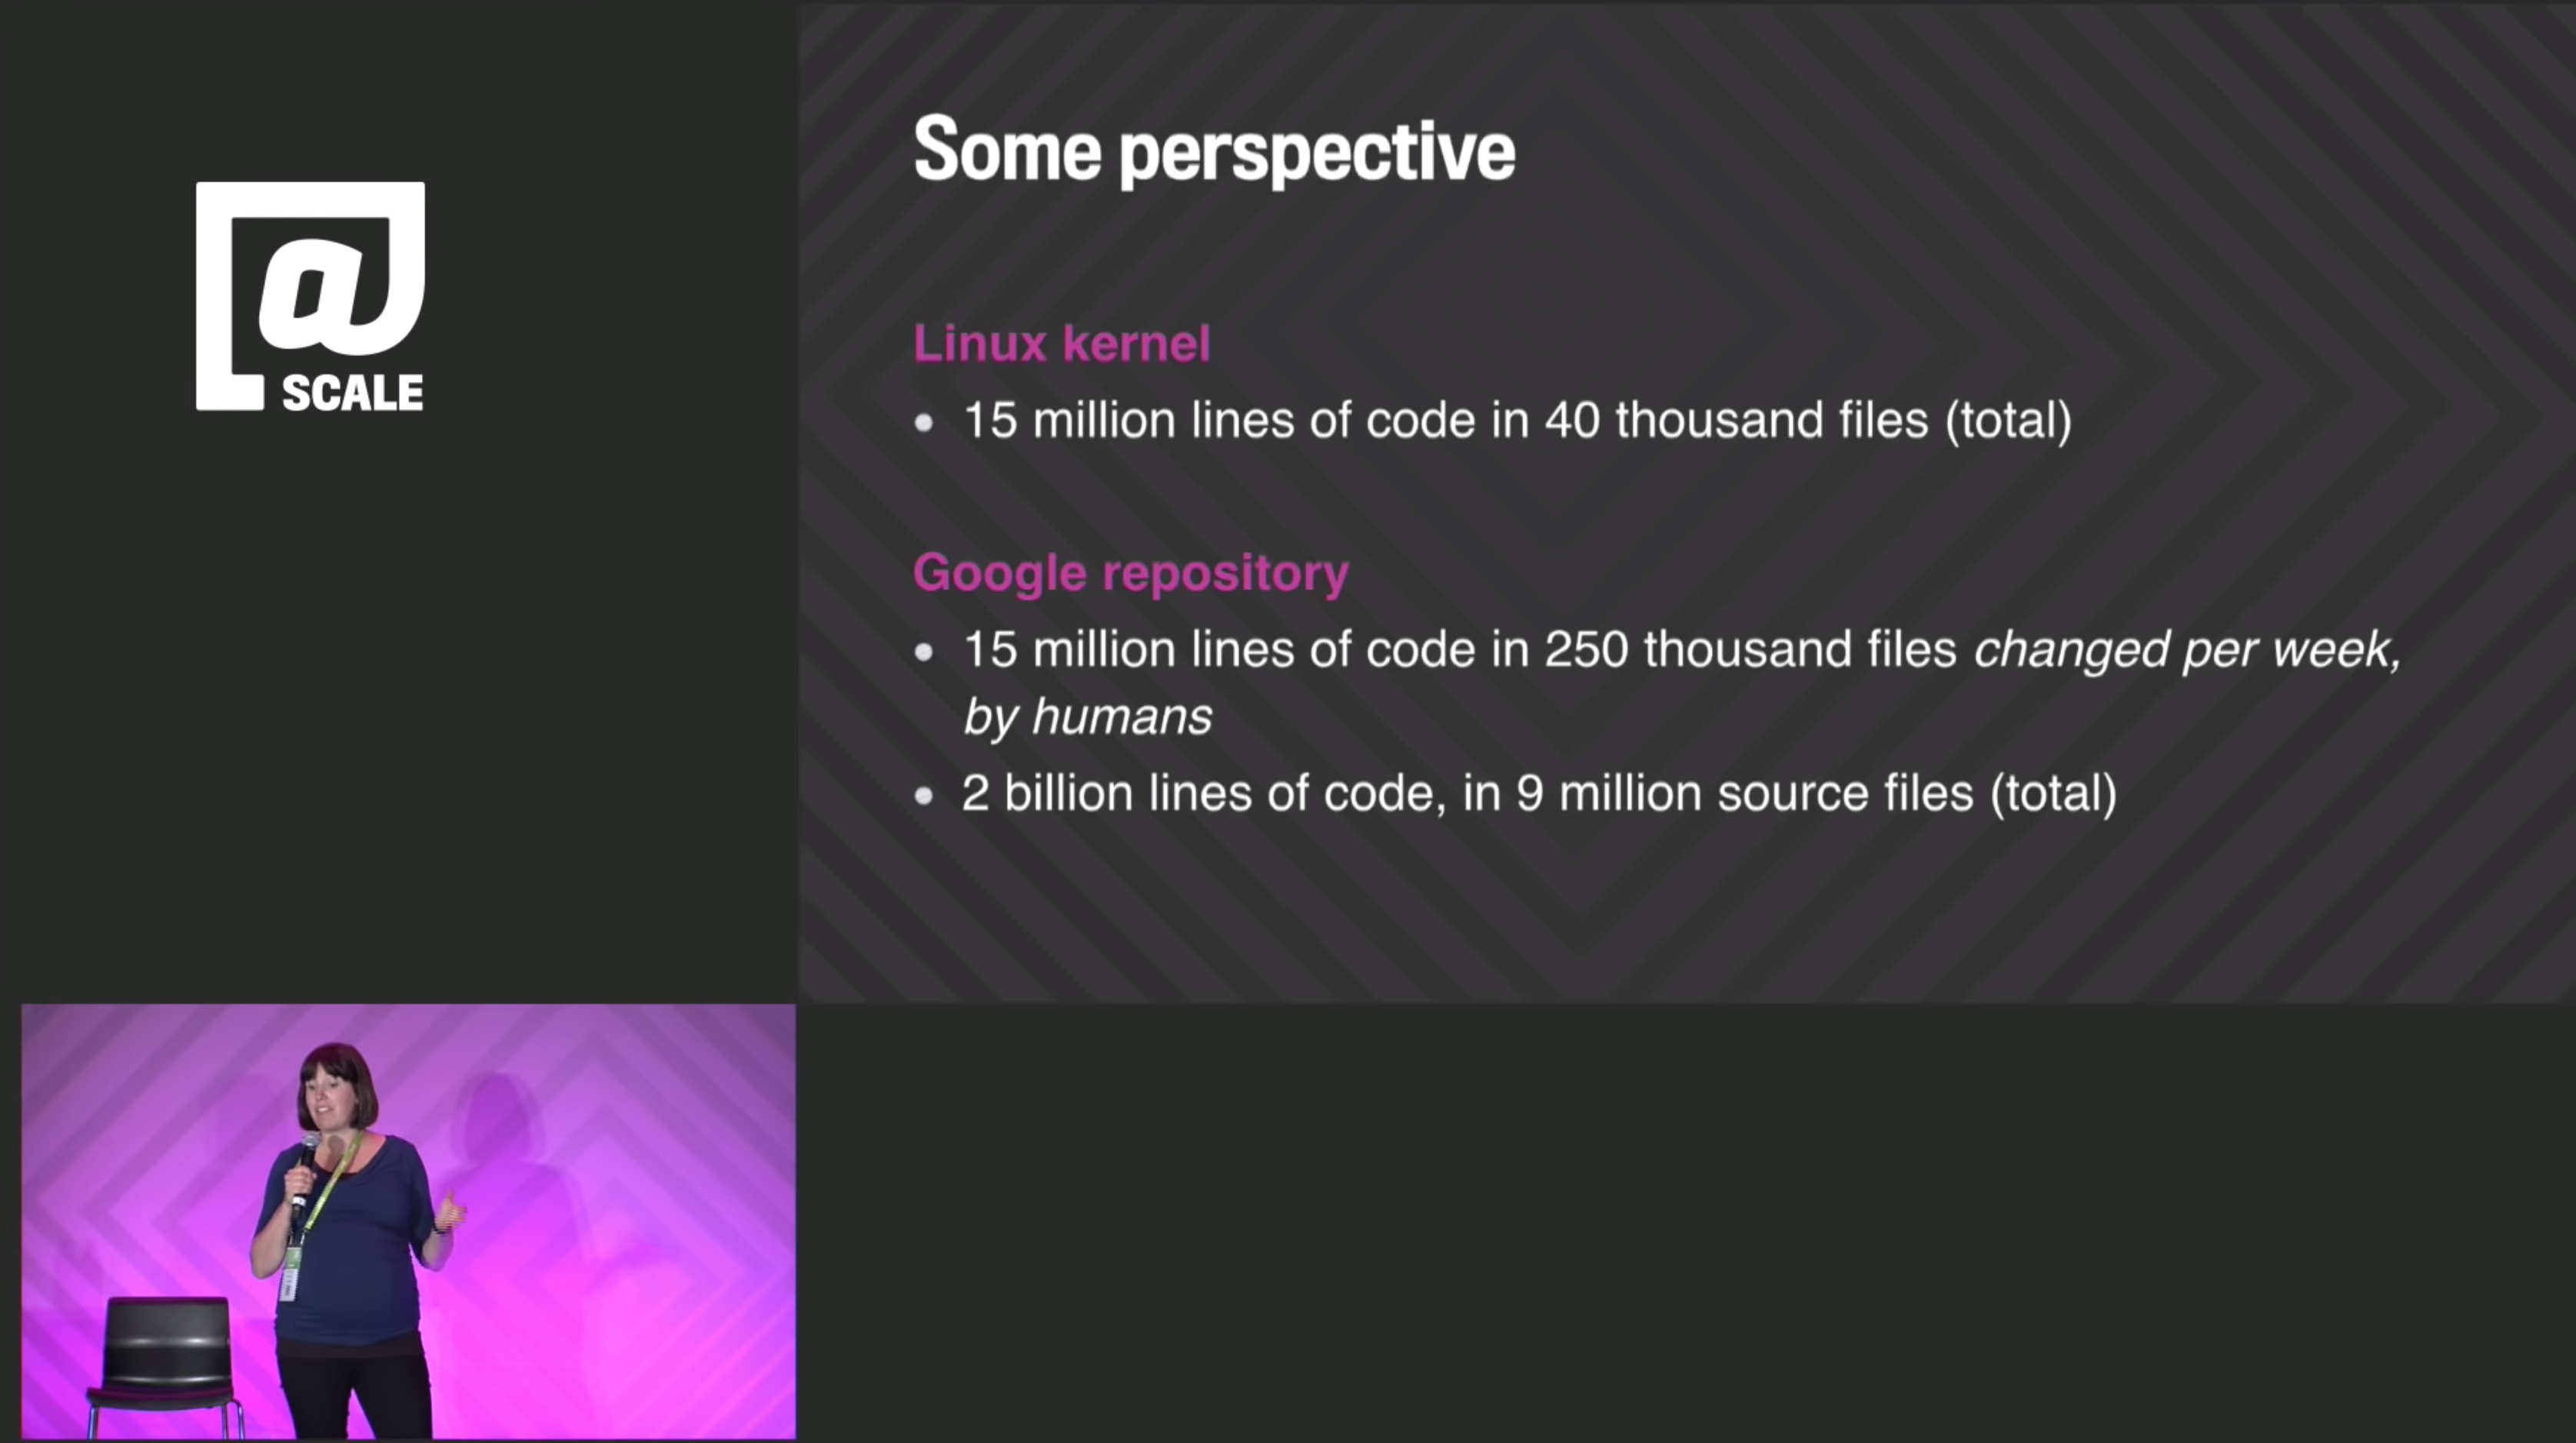
\includegraphics[width=\linewidth,height=0.6\textheight,keepaspectratio]{chapters/02_computer_science/figures/google/programming/loc.png}
                \caption{Größe der Google Codebasis \cite{google:potvin}}
                \label{fig:my_label}
            \end{figure}
        \end{column}
        \begin{column}{0.4\textwidth}
            \begin{figure}
            \centering
            \begin{subfigure}{0.475\textwidth}
                \centering
                
\includegraphics[width=\textwidth,height=0.15\textheight,keepaspectratio]{chapters/02_computer_science/figures/google/programming/languages/python.png}
            \end{subfigure}
            \begin{subfigure}{0.475\textwidth}
                \centering
                
\includegraphics[width=\textwidth,height=0.15\textheight,keepaspectratio]{chapters/02_computer_science/figures/google/programming/languages/cpp.png}
            \end{subfigure}
            
            \vskip\baselineskip
            
            \begin{subfigure}{0.475\textwidth}
                \centering
                
\includegraphics[width=\textwidth,height=0.15\textheight,keepaspectratio]{chapters/02_computer_science/figures/google/programming/languages/java.png}
            \end{subfigure}
            
             \begin{subfigure}{0.475\textwidth}
                \centering
                
\includegraphics[width=\textwidth,height=0.15\textheight,keepaspectratio]{chapters/02_computer_science/figures/google/programming/languages/go.png}
            \end{subfigure}
            
            \caption{Hauptprogrammiersprachen von Google}
            \end{figure}
        \end{column}
    \end{columns}
    \end{frame}
    
    
    \begin{frame}[fragile]{Was ist Informatik?}
        \framesubtitle{Beispiel Google: Systems Design}
        \begin{figure}
            \centering
            
\includegraphics[width=\linewidth,height=0.3\textheight,keepaspectratio]{chapters/02_computer_science/figures/google/sys_des/searches.png}
            \caption{
                Google-Anfragen pro Jahr (2016, geschätzt) 
                \cite{google:sys_des:searches}
            }
        \end{figure}
        
        \begin{figure}
            \centering
            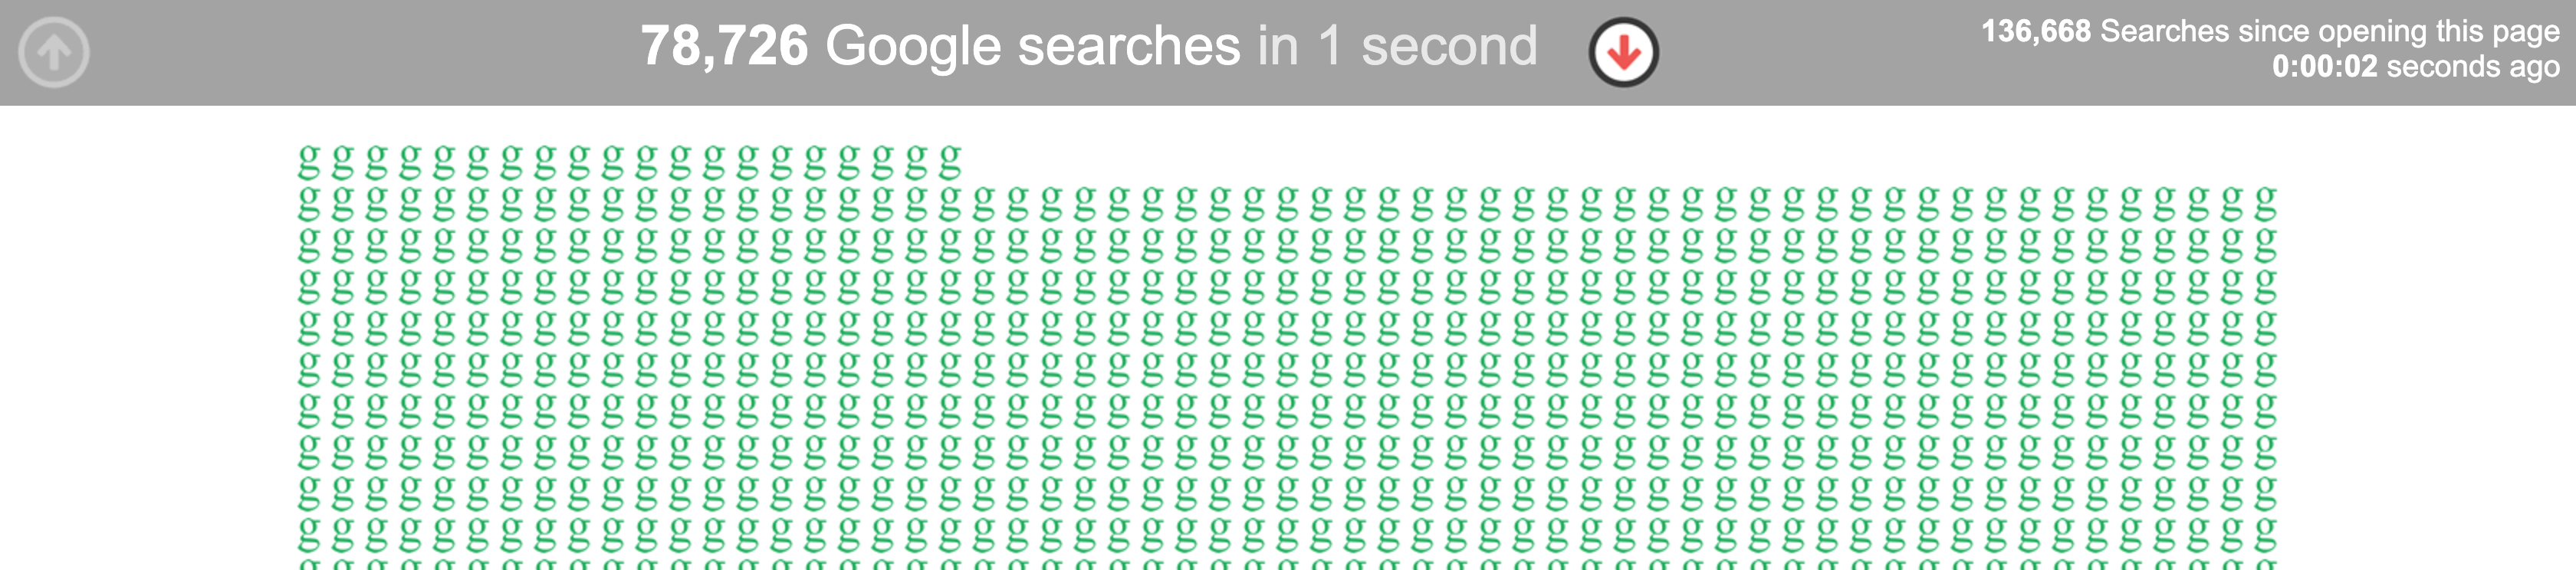
\includegraphics[width=\linewidth,height=0.3\textheight,keepaspectratio]{chapters/02_computer_science/figures/google/sys_des/searches2.png}
            \caption{
                \href{https://www.internetlivestats.com/one-second/#google-band}{Visualisierung der Anzahl der Google-Suchen pro Sekunde} (geschätzt)
            }
        \end{figure}
    
    \end{frame}
    
     \begin{frame}{Was ist Informatik?}
        \framesubtitle{Beispiel Google: Systems Engineering}
        \begin{figure}
            %\centering
            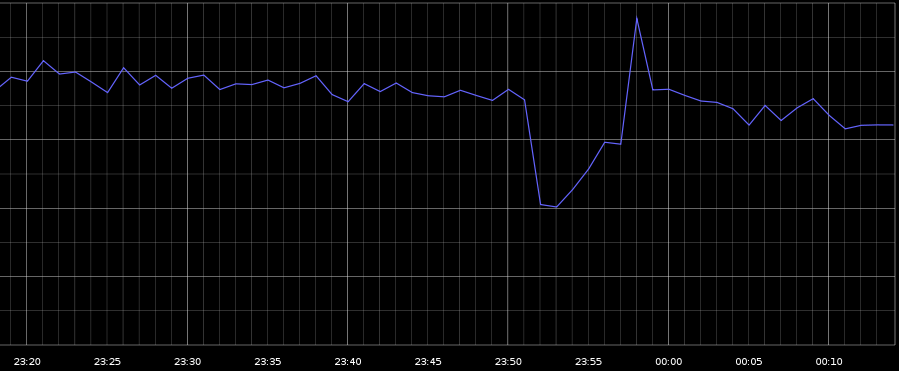
\includegraphics[width=\linewidth,height=0.3\textheight,keepaspectratio]{chapters/02_computer_science/figures/google/downtime/downtime.png}
            \caption{Einbruch des Internettraffics um 40\% während eines 2-minütigen Ausfalls von Google \cite{google:down:chart}}
            \label{fig:my_label}
        \end{figure}
        
         \begin{figure}
            %\centering
            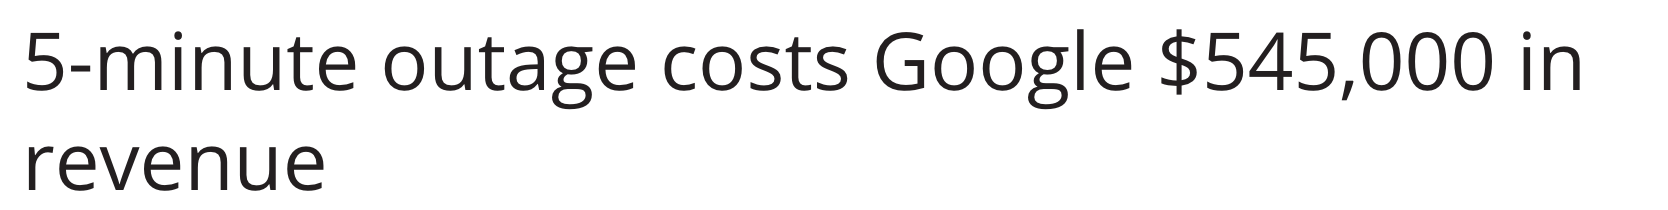
\includegraphics[width=0.4\linewidth,height=0.3\textheight,keepaspectratio]{chapters/02_computer_science/figures/google/downtime/costs.png}
            \caption{Geschätzte Kosten des Google-Ausfalls \cite{google:down:costs}}
            \label{fig:my_label}
        \end{figure}
    \end{frame}
    
    
    \begin{frame}{Was ist Informatik?}
        \framesubtitle{Beispiel Google: Algorithmik, Komplexitätsanalyse \& Mathematik}
        \begin{figure}
            \centering
            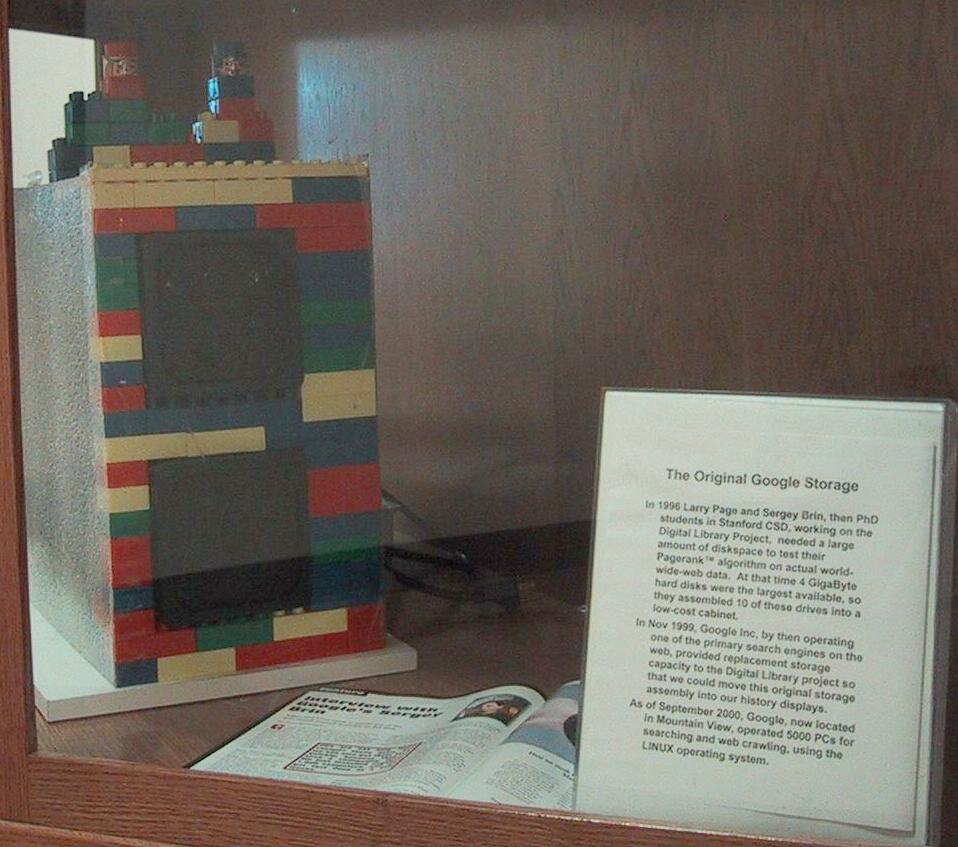
\includegraphics[width=\linewidth,height=0.6\textheight,keepaspectratio]{chapters/02_computer_science/figures/google/storage.jpg}
            \caption{Der erste Google-Computer mit 10x4 GB Harddrives \cite{google:alg:storage}}
            \label{fig:my_label}
        \end{figure}
      
    \end{frame}
    
    
    \begin{frame}{Was ist Informatik?}
        \framesubtitle{Beispiel Google: Algorithmik, Komplexitätsanalyse \& Mathematik}
        \begin{figure}
            \centering
            
\includegraphics[width=\linewidth,height=0.6\textheight,keepaspectratio]{chapters/02_computer_science/figures/google/algorithms/results.png}
            \caption{Leistungsfähigkeit der Google-Suche}
            \label{fig:my_label}
        \end{figure}
        
        \begin{quote}
            "Der Google-Suchindex umfasst Milliarden von Webseiten und ist über 100.000.000 Gigabyte groß." \cite{google:alg:index}
        \end{quote}
    \end{frame}
    
    \begin{frame}{Was ist Informatik?}
        \framesubtitle{Beispiel Google: Systemarchitektur}
        \begin{figure}
            \centering
            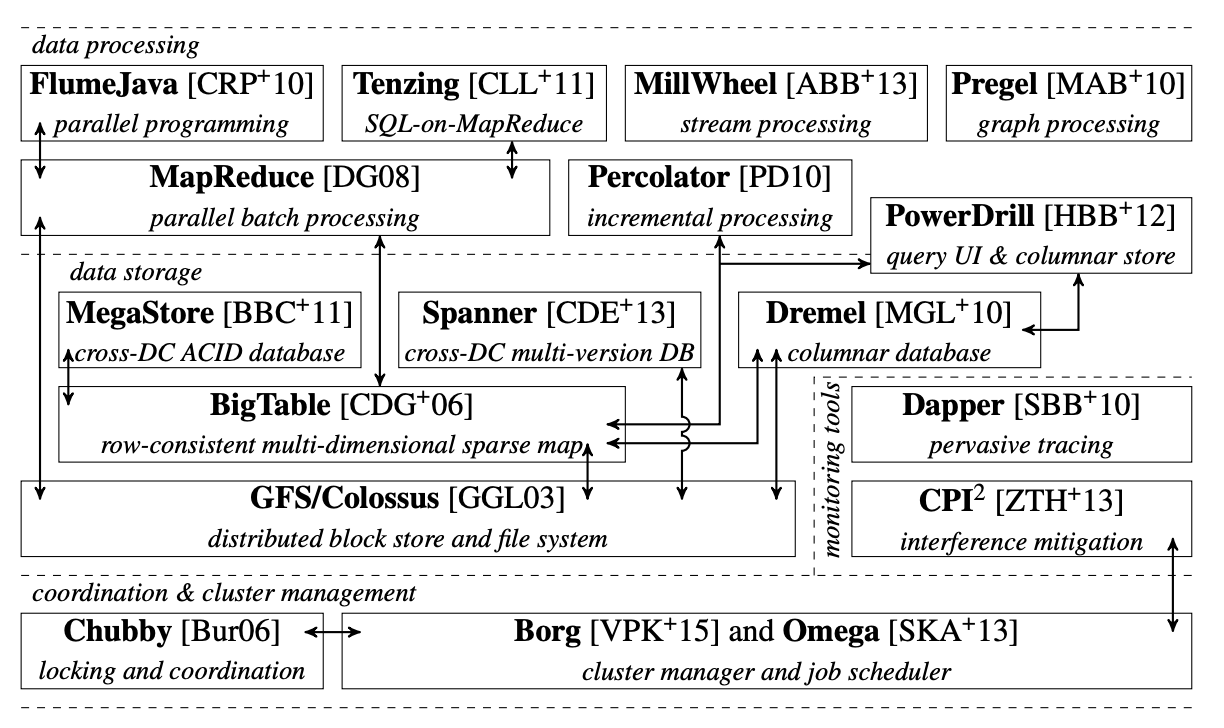
\includegraphics[width=\linewidth,height=0.6\textheight,keepaspectratio]{chapters/02_computer_science/figures/google/architecture/stack.png}
            \caption{Der Google Infrastruktur-Stack \cite{google:arch:stack}}
            \label{fig:my_label}
        \end{figure}
        
        
    \end{frame}
    
    
    \begin{frame}{Was ist Informatik?}
        \framesubtitle{Beispiel Google: Verteilte Systeme}
        \begin{figure}
            \centering
            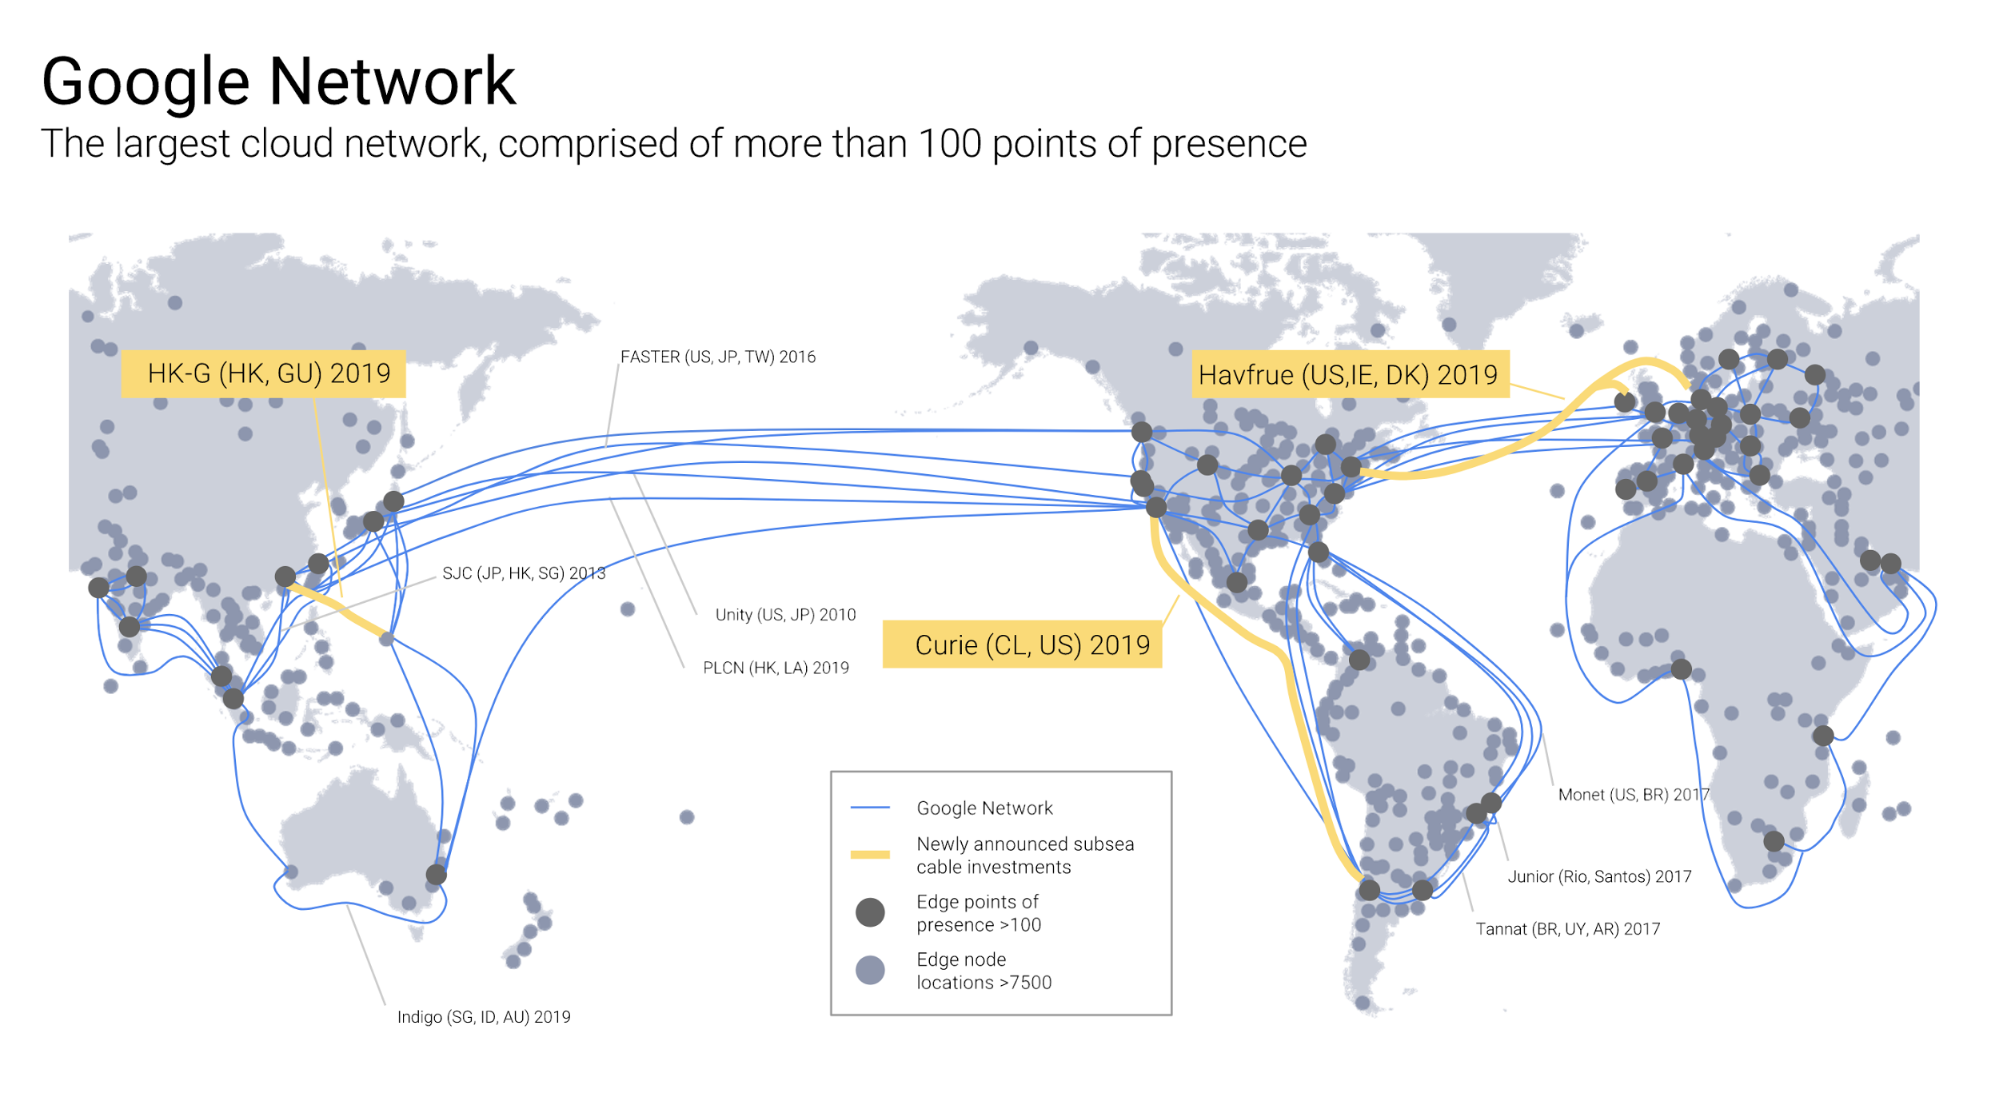
\includegraphics[width=\linewidth,height=0.3\textheight,keepaspectratio]{chapters/02_computer_science/figures/google/distributed/infrastructure.png}
            \caption{Globale Netzwerk-Infrastruktur der Google Cloud \cite{google:dist:infra}}
            \label{fig:my_label}
        \end{figure}
        
        \begin{figure}
            \centering
            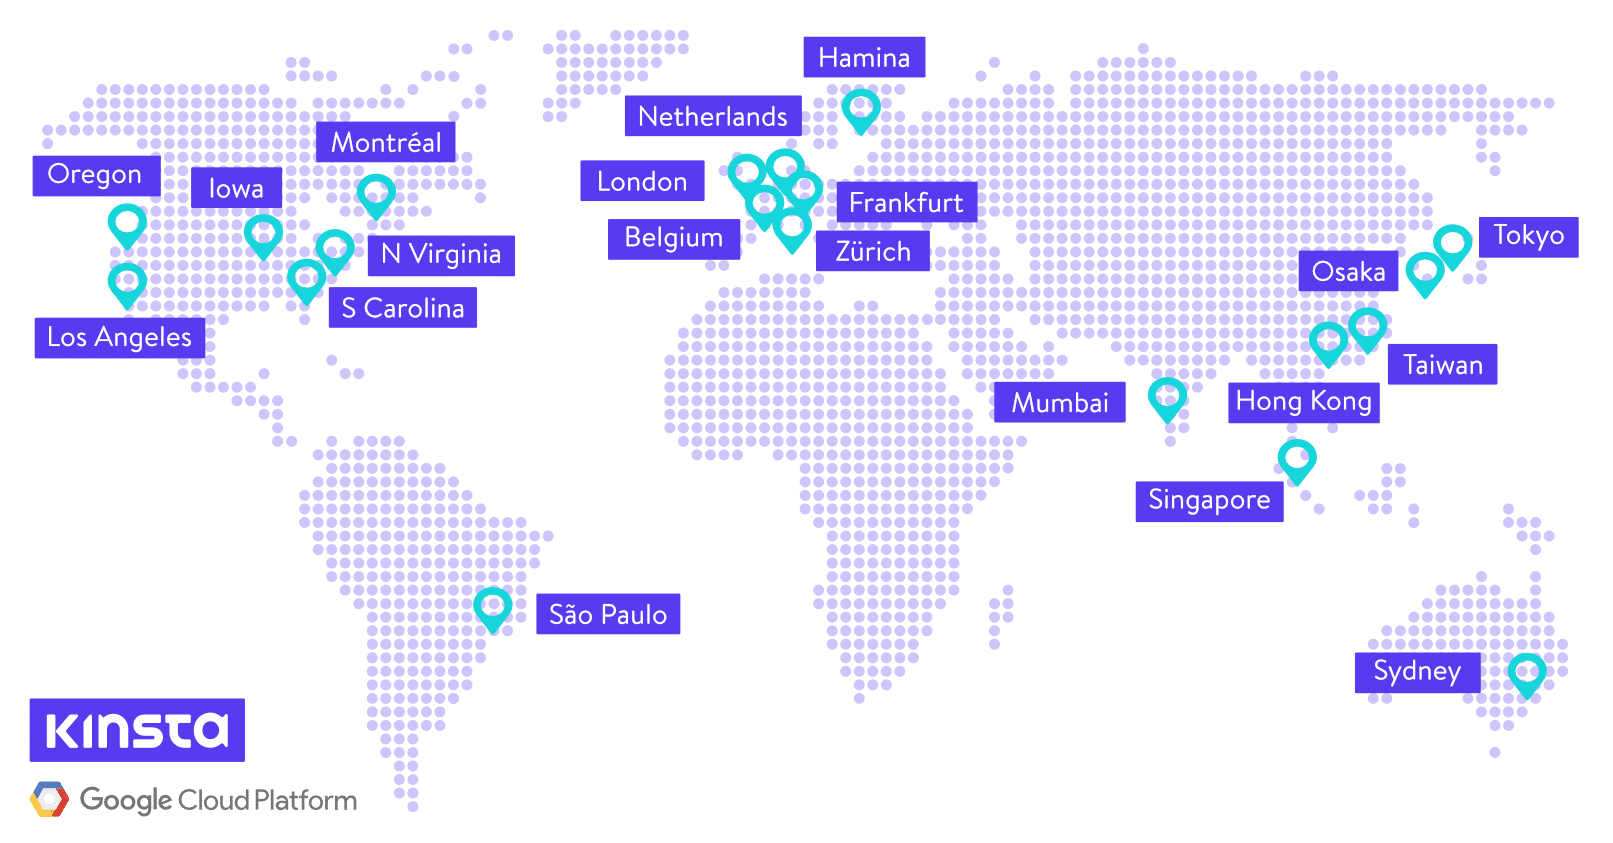
\includegraphics[width=\linewidth,height=0.3\textheight,keepaspectratio]{chapters/02_computer_science/figures/google/distributed/datacenter.png}
            \caption{Standorte der Google-Rechenzentren \cite{google:dist:datacenter}}
            \label{fig:my_label}
        \end{figure}
        
        
    \end{frame}

    \subsection{Disziplinen der Informatik} 
    
    \begin{frame}{Was ist Informatik?}
        \framesubtitle{Disziplinen der Informatik}
        Informatik besteht aus vielen Teildisziplinen, z.B.:
        \begin{itemize}
            \item Computerarchitektur
            \item Rechnernetze
            \item Compilerentwurf- und entwicklung
            \item Theoretische Informatik
            \item Verteilte Systeme
            \item Simulation \& Computergrafik
            \item Künstliche Intelligenz \& Machine Learning
            \item ...
        \end{itemize}
    \end{frame}
    
    \begin{frame}{Was ist Informatik?}
        \framesubtitle{Disziplinen der Informatik}
        \begin{figure}
            \centering
            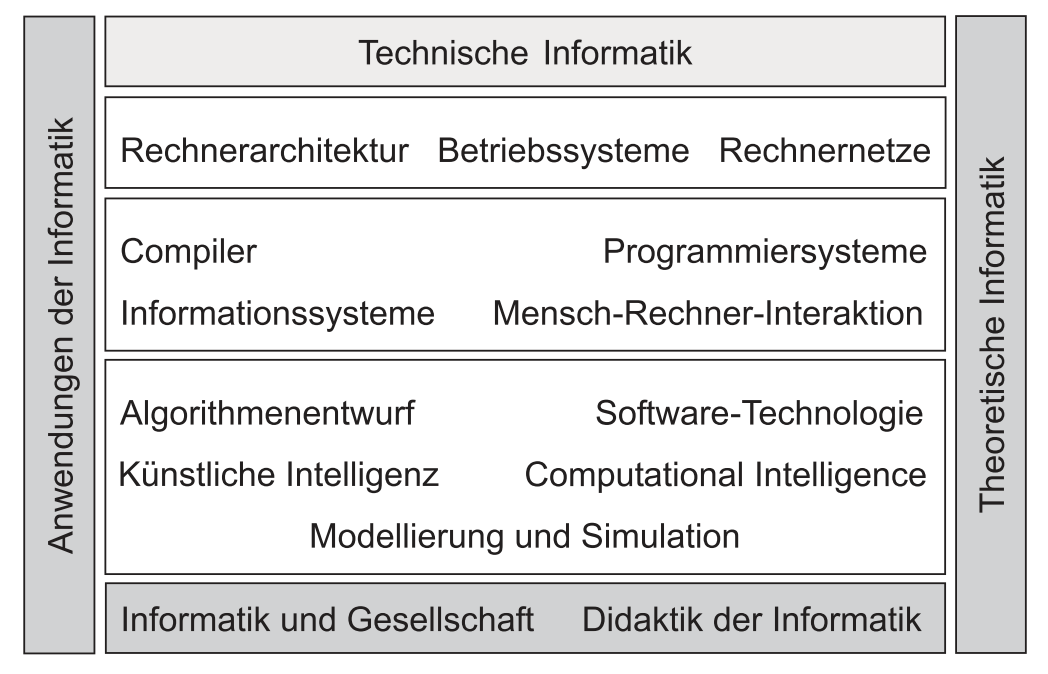
\includegraphics[width=\linewidth,height=0.6\textheight,keepaspectratio]{chapters/02_computer_science/figures/informatik_einordnung.png}
            \caption{Einordnung der Teilgebiete der Informatik \cite{Muller2015}}
            \label{fig:my_label}
        \end{figure}
    \end{frame}
        
    